\documentclass[12pt,twoside,a4paper]{book}


\usepackage[utf8]{inputenc}
\usepackage[T1]{fontenc}
\usepackage{lmodern}
\usepackage{amsmath,amssymb,amsthm}
\usepackage{mathabx}\changenotsign
\usepackage{mathrsfs}
\usepackage{dsfont}
\usepackage[babel]{microtype}
\usepackage{xcolor}  	
\usepackage[backref]{hyperref}
\usepackage{mathtools}
\usepackage{indentfirst}
\usepackage{graphicx} % Gerencia imagens incluidas
\usepackage{float} 

\hypersetup{
	colorlinks,
    linkcolor={red!60!black},
    citecolor={green!60!black},
    urlcolor={blue!60!black},
}

\usepackage{bookmark}

\usepackage[abbrev,msc-links,backrefs]{amsrefs}
\usepackage{doi}
\renewcommand{\doitext}{DOI\,}

\renewcommand{\PrintDOI}[1]{\doi{#1}}

\renewcommand{\eprint}[1]{\href{http://arxiv.org/abs/#1}{arXiv:#1}}


\usepackage[T1]{fontenc}
\usepackage{lmodern}

\usepackage[english]{babel}
\numberwithin{equation}{section}

\linespread{1.3}
\usepackage{amsfonts}
\usepackage{geometry}
\geometry{left=27.5mm,right=27.5mm, top=25mm, bottom=25mm}


\usepackage{enumitem}
\def\rmlabel{\upshape({\itshape \roman*\,})}
\def\RMlabel{\upshape(\Roman*)}
\def\alabel{\upshape({\itshape \alph*\,})}
\def\Alabel{\upshape({\itshape \Alph*\,})}
\def\nlabel{\upshape({\itshape \arabic*\,})}

\def\aplabel{\upshape({\itshape \alph*\,$'$})}

\let\polishlcross=\l
\def\l{\ifmmode\ell\else\polishlcross\fi}

\def\tand{\ \text{and}\ }
\def\qand{\quad\text{and}\quad}
\def\qqand{\qquad\text{and}\qquad}

\let\emptyset=\varnothing
\let\setminus=\smallsetminus
\let\backslash=\smallsetminus
%\let\subset\subseteq
\let\log=\ln

\newcommand\mc{\mathop{\textrm{\rm mc}}\nolimits}

\makeatletter
\def\moverlay{\mathpalette\mov@rlay}
\def\mov@rlay#1#2{\leavevmode\vtop{   \baselineskip\z@skip \lineskiplimit-\maxdimen
   \ialign{\hfil$\m@th#1##$\hfil\cr#2\crcr}}}
\newcommand{\charfusion}[3][\mathord]{
    #1{\ifx#1\mathop\vphantom{#2}\fi
        \mathpalette\mov@rlay{#2\cr#3}
      }
    \ifx#1\mathop\expandafter\displaylimits\fi}
\makeatother

\DeclareMathOperator{\dom}{{\rm dom}}

\newcommand{\dcup}{\charfusion[\mathbin]{\cup}{\cdot}}
\newcommand{\bigdcup}{\charfusion[\mathop]{\bigcup}{\cdot}}


\DeclareFontFamily{U}  {MnSymbolC}{}
\DeclareSymbolFont{MnSyC}         {U}  {MnSymbolC}{m}{n}
\DeclareFontShape{U}{MnSymbolC}{m}{n}{
    <-6>  MnSymbolC5
   <6-7>  MnSymbolC6
   <7-8>  MnSymbolC7
   <8-9>  MnSymbolC8
   <9-10> MnSymbolC9
  <10-12> MnSymbolC10
  <12->   MnSymbolC12}{}
\DeclareMathSymbol{\powerset}{\mathord}{MnSyC}{180}



\makeatletter
\def\namedlabel#1#2{\begingroup
    #2%
    \def\@currentlabel{#2}%
    \phantomsection\label{#1}\endgroup
}
\makeatother


\newtheorem{theorem}             {Theorem}[section]
\newtheorem{lemma}     	[theorem] {Lemma}
\newtheorem{conjecture}	[theorem] {Conjecture}
\newtheorem{property}  	[theorem] {Property}
\newtheorem{definition}	[theorem] {Definition}
\newtheorem{proposition}[theorem] {Proposition}
\newtheorem{corollary}	[theorem] {Corollary}
\newtheorem{fact}	[theorem] {Fact}
\newtheorem{claim}	[theorem] {Claim}

\newtheoremstyle{remark}  {2pt}  {4pt}  {\rm}  {}  {\bfseries}  {.}  {.3em}          {}
\theoremstyle{remark}
\newtheorem{remark}	[theorem] {Remark}
\newtheorem{example}	[theorem] {Example}

\renewcommand{\thefootnote}{\fnsymbol{footnote}}

\let\eps=\varepsilon
\let\theta=\vartheta
\let\rho=\varrho
\let\phi=\varphi


\def\NN{\mathds N}
\def\ZZ{\mathds Z}
\def\QQ{\mathds Q}
\def\RR{\mathds R}
\def\PP{\mathds P}
\def\EE{\mathds E}

\def\cB{\mathcal B}
\def\cR{\mathcal R}

\def\ra{\longrightarrow}
\usepackage{centernot}
\def\nra{\centernot\longrightarrow}
\def\red{\text{\rm red}}
\def\blue{\text{\rm blue}}
\def\green{\text{\rm green}}
\def\R{\text{\rm red}}
\def\B{\text{\rm blue}}

\usepackage{datetime}
\usepackage{lineno}
\newcommand*\patchAmsMathEnvironmentForLineno[1]{%
\expandafter\let\csname old#1\expandafter\endcsname\csname #1\endcsname
\expandafter\let\csname oldend#1\expandafter\endcsname\csname end#1\endcsname
\renewenvironment{#1}%
{\linenomath\csname old#1\endcsname}%
{\csname oldend#1\endcsname\endlinenomath}}%
\newcommand*\patchBothAmsMathEnvironmentsForLineno[1]{%
\patchAmsMathEnvironmentForLineno{#1}%
\patchAmsMathEnvironmentForLineno{#1*}}%
\AtBeginDocument{%
\patchBothAmsMathEnvironmentsForLineno{equation}%
\patchBothAmsMathEnvironmentsForLineno{align}%
\patchBothAmsMathEnvironmentsForLineno{flalign}%
\patchBothAmsMathEnvironmentsForLineno{alignat}%
\patchBothAmsMathEnvironmentsForLineno{gather}%
\patchBothAmsMathEnvironmentsForLineno{multline}%
}
\usepackage{graphicx}
\begin{document}
%\linenumbers

%\title{Extremal and Probabilistic Combinatorics}

\begin{center}
{\bf Extremal and Probabilistic Combinatorics}\\
\vspace{2cm}
Diogo Eduardo Lima Alves\\
\vspace{3cm}

PROJETO DE GRADUAÇÃO EM COMPUTAÇÃO PRESENTED\\
TO\\
CENTRO DE MATEMÁTICA, COMPUTAÇÃO E COGNIÇÃO\\
OF\\
UNIVERSIDADE FEDERAL DO ABC\\
FOR\\
OBTAINING TITLE\\
OF\\
BACHAREL EM CIÊNCIA DA COMPUTAÇÃO\\
\vspace{4cm}
Advisor: Prof. Dr. Guilherme Oliveira Mota\\
\vfill
Santo André, Agosto de 2018
\end{center}

\tableofcontents
\listoffigures
%\listoftables

\chapter{Introduction}
Computer Science is truly fundamental for the fast development of Science in the last century, also being fundamental for its validation and communication. It is really hard to think about actual Science without the use of computers or strong science communities connected and accessible by the internet. Computer Science is also essential for the business. All multinational company is also a software company since the way of production, operating and delivering products are managed by software and these aspects are determinants for the success level of any company in the world, it is also not uncommon that one of the most valuable assets of a company can be connected to data, software and algorithms. In this scenario, graphs are also very interesting due its importance to Computer Science.

Graphs are one of the most flexible structures, even for math theory either for efficient algorithms, impacting the study of Algebra, Probability and Combinatorics. They can be used even for modeling many real scenarios in a very easy understandable graphical scheme whose properties can be explored to obtain many useful information what explains its huge importance for many knowledge areas not directly connected to Computer Science or Math Theory.   

This project, more specifically, focus on classical results of Extremal Combinatorics Theory and Graph Theory. It has detailed ideas and explanations about theorems and concepts of a large period of time which have already been intensively studied.

Extremal Combinatorics studies the maximum or minimum size a collection of objects can be at the same time it satisfies certain restrictions. Here these objects will be focus on graphs and graphs' substructures. 

Ramsey Theory is the study of finding order in chaos and, in general, solves mathematical equations in the integers.

Extremal Graph Theory studies graphs' size, as the number interval of edges and vertices, since a specific substructure is forbidden inside the main graph.

The Probabilistic Method is a very useful tool for solving problems in many areas, because it is flexible and uses a random graph which is simple to use and work with the probabilities that makes possible prove statements with high or not null probability.

%\chapter{Justification}
%ME INTERESSEI PELO TEMA, APENAS!


%\chapter{Objectives}



%\chapter{Methodology}
%The main bibliography referential material used in this project is the book ``Extremal and Probabilistic Combinatorics'' written by Robert Morris and Roberto Imbuzeiro Oliveira which is part of Impa's mathematical publications and is a result of a Extremal Combinatorics course.

%Almost all the doubts and problems about proofs, explanations and structure over the entire text construction was supported by the projects' advisor, the professor Dr. Guilherme Oliveira Mota.



\chapter{Ramsey Theory}

Ramsey's theory is especially philosophical among the components of the extremal combinatorics. Ramsey's theory wants to find order in chaos, that is, it is motivated by the thought that complete chaos or complete order is impossible to achieve, then we can always have a piece of information independent of the complexity or particular characteristics of any graph.

\section{Ramsey's Theorem}
Consider the following question:
``Given a group of 6 people, are there 3 people that are mutual friends or 3 people are mutual strangers?''

It is possible to suppose without loss of generality that Richard knows at least three people, Maria, Bete and Jack. If any pair of these friends know each other, then it is formed a friendly triangle, otherwise Maria, Bete and Jack form a unfriendly triangle themselves. Replacing people with vertices and a friend relationship with colours (blue for friends and red otherwise) we realize that with 6 peoples we always have a monochromatic triangle independently of the colouring, but what about 5 people?

\begin{definition}\label{def:RamseyNumbers} 
The minimum $n$ such that any $2$-colouring on $K_n$ induces a complete subgraph $K_s$ whose edges are monochromatic in color $1$ or a complete subgraph $K_t$ whose edges are monochromatic in color $2$ is the Ramsey Number $R(s,t)$.
\end{definition}

The $K_5$ can be constructed without a monochromatic triangle as Figure \ref{fig:K5}, this shows that Ramsey number cannot be less than 6, what can be written as  R(3,3) = 6.

\begin{figure}[H]
     \centering
     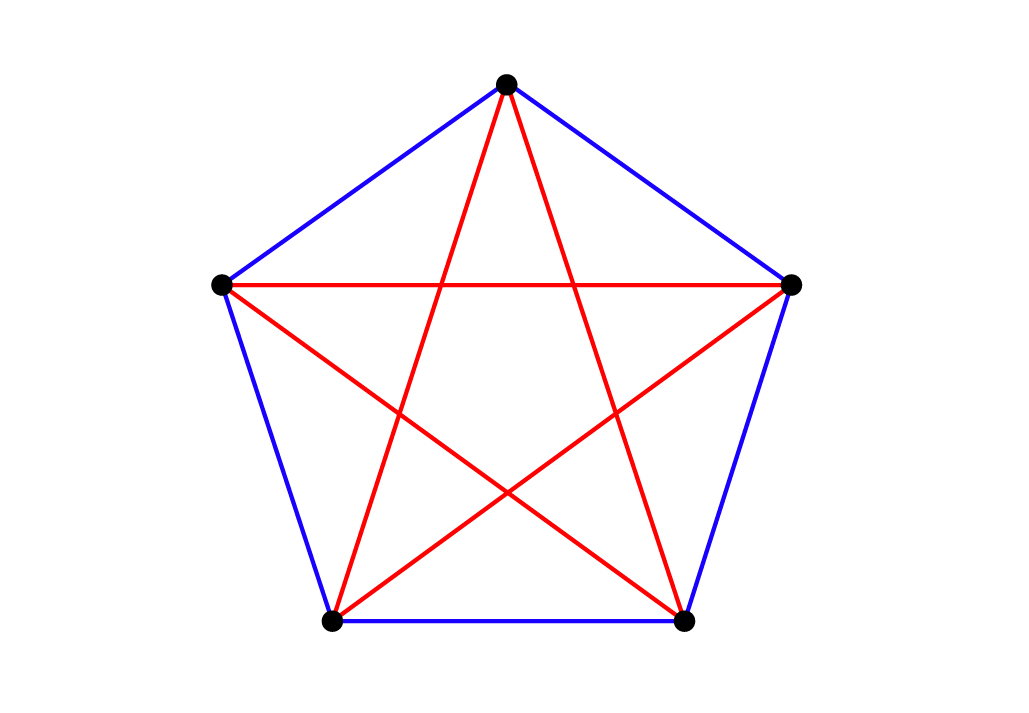
\includegraphics[scale=1]{Figuras/K5-sem-triangulo.jpg}
     \caption{$K_5$ without monochromatic triangle.}
     \label{fig:K5}
\end{figure}

\begin{theorem}\label{thm:RamseyTheorem} 
(Ramsey's Theorem). Let $r \geq 1$ be an integer. Every colouring $c\colon \dbinom{\mathbb{N}}{2}$ $\rightarrow$ $[r]$ of the pairs in $\mathbb{N}$ contains an infinite monochromatic subset of pairs.
\end{theorem}

In order to prove this theorem, it is needed only the pigeonhole principle as it follows:

``If a infinite number of letters lie in a finite number of pigeonholes, then some pigeonhole must contain an infinite number of letters''

Imagine we have a finite number of parts to divide $\mathbb{N}$ whose elements are infinite, let the number of parts be r. We can start giving part 1 a finite quantity of elements, doing the same for parts $\{2, 3,..., r-1\}$. So at this point we have $\{1,2,3,...,r-1\}$ being a set of parts with a finite number of elements, but |$\mathbb{N}$| = $\infty$ and once $|\{1, 2, 3,..., r-1\}|$ is finite we still have infinite elements and only one part to use, so at least one of these parts must have infinite elements.

Given a colouring $c\colon\dbinom{\mathbb{N}}{2}$ $\rightarrow$ $[r]$, being $i$ a colour and  $v$ a vertex $\in \mathbb{N}$, define $N_i(v) =\{ w: c(vw)=i\}$ , can be read as the colour $i$ neighbourhood of $v$.

\section{Schur's Theorem}

\begin{theorem}\label{thm:Schur'sTheorem}
(Schur's Theorem, 1916). Considering any colouring $c\colon \mathbb{N} \rightarrow [r]$, it implies a monochromatic $x,y,z$ with the property $x+y=z$.
\end{theorem}
\begin{proof}
  For a vertex colouring  given as $c\colon \mathbb{N} \rightarrow [r]$ define a edge colouring $c'\colon \binom{\mathbb{N}}{2} \rightarrow [r]$ as $c'(\{a,b\}) \coloneqq c(|a-b|)$. By Theorem~\ref{thm:RamseyTheorem}, there exists a monochromatic triangle with three vertices, say $\{x,y,z\}$, with $x<y<z$.\\
Using the definition of $c'$  we have
$$c'({x,y}) = i = c(|y-x|)$$
$$c'({x,z})=  i = c(|z-x|)$$
$$c'({y,z}) = i = c(|z-y|)$$

From that, $c(|y-x|) = c(|z-x|) = c(|z-y|)$, and $(z-y)+(y-x)=(z-x)$ forms a monochromatic $x,y,z$ such that $x+y=z$, as required.\\
\end{proof}

\section{Finite Ramsey's Theorem}

\begin{theorem}\label{thm:ErdosandS}
(Erd\H{o}s and Szekeres, 1935; Erd\H{o}s, 1947).\\
$$(\sqrt{2})^k \ll R(k) \ll 4^k.$$
\end{theorem}
\begin{proof} We start by proving the upper bound. Considering every $k, \ell \in \mathbb{N}$ we assume:\\
$$R(k,\ell ) \leq R(k-1,\ell )+R(k,\ell-1).$$\\
Choose $n \geq R(k-1,\ell) + R(k, \ell-1)$ and pick any vertex $v$ from $[n]$. Using Pigeonhole principle we realize $v$ has either at least $R(k-1,\ell)$ red neighbours, or at least $R(k,\ell-1)$ blue neighbours, for simplicity assume that $v$ has at least $R(k-1,\ell)$ red neighbours. By definition we have on the red neighbors of $v$ a red $K_{k-1}$ or a blue $K_{\ell}$, if it is a $K_{\ell}$ we are done and if it is a $K_{k-1}$ we can add $v$, forming a $K_k$. We just proved we always have a $K_k$ red or a $K_{\ell}$ blue with such $n$ and it is a upper bound for equation $R(k,\ell) \leq R(k-1,\ell)+R(k,\ell-1)$ because it doesn't prove this $n$ is the minimum one, only shows that for this specific $n$ it is true.\\
By induction hypothesis:
$$R(k,\ell) \leq \binom{k+\ell - 2}{k - 1}.$$
This implies on:
$$R(k-1,\ell)\leq \binom{k+\ell -3}{k-2},$$ and $$R(k,\ell-1)\leq \binom{k+\ell-3}{\ell-1}.$$
By Pascal's rule $\binom{n-1}{k} + \binom{n-1}{k-1} = \binom{n}{k}$ we have:

$$R(k,\ell)\leq \binom{k-1+\ell}{k-1} + \binom{k+\ell-1}{\ell-1} = \binom{k+ \ell -2}{k-1}.$$
Confirming our induction hypothesis. Now let $k = \ell$ and using Stirling's approximation for binomial coefficient $\binom{2n}{n} \approx (2^{2n}/\sqrt{\pi n})$, assuming $n$ is sufficiently large follows:

\begin{align*}
R(k) &\leq \binom{2k -2}{k-1}\\
& \approx \frac{2^{2k-2}}{\sqrt{\pi (k-1)}}\\
& \ll 4^k.
\end{align*}

Finishing the upper bound proof.\\

It is hard to find colourings whose subgraphs are not big and not monochromatic, this is counter-intuitive but is really hard to construct this type of graph. However, in 1947 Erd\H{o}s made a important contribution for combinatorics showing a simple proof of an exponential lower bound on $R(k)$.

Now we proceed by proving the lower bound. Given a random coloring $c\colon \binom{n}{2} \rightarrow \{0,1\}$ let $1/2$ be the probability of a red $c(i)(j)$ for any edge $ij$ in $e(K_n)$.\\ 
Define X as the number of monochromatics cliques in $K_n$. The expected value for $X$ is $\binom{n}{k}$ times the probability of a given clique be monochromatic, then:
$$\binom{n}{k}\frac{1}{2} ^{\binom{k}{2}-1} \leq 2 \left( \frac{en}{k} \left( \frac{1}{\sqrt{2}} \right)^{k-1} \right)^{k} \ll 1.$$ 
This holds if: 
\begin{align*}
n &<\frac{1}{e\sqrt{2}}k2^{k/2} \\
& = \frac{k(\sqrt{2})^{k}}{e\sqrt{2}}\\
& \gg (\sqrt{2})^k.
\end{align*}

Since the expected value for $X$ is less than $1$, then there must exist a colouring in which $X=0$, thus the proof is finished.
\end{proof}

\section{Van der Waerden's Theorem}

\begin{theorem} (Van der Waerden, 1927). For every $\mathbb{N}$ colouring with any $r$ colours it contains arbitrarily long monochromatic arithmetic progressions. 
\end{theorem}

\begin{proof}To prove this theorem we need the following definition,

\begin{definition}
$W(r,k) =$ min $\{n \colon \forall c \colon [n] \rightarrow \{1,...,r\}$ exists a monochromatic arithmetic  progression of length $k$ for all $r$ and $k$ in $\mathbb{N}\}$.
\end{definition}

We claim that $W(r,k)$ exists and we prove it by double induction, so assume that $W(r, k-1)$ exists. Note if $k \leq 2$ the result is trivial.

First denote the arithmetic progression $\{a, a + d, a +2d, ..., a+(k-1)d\}$ by AP$(a,d,k)$ such that it has common difference  $d$ and length $k$.

We say arithmetic progressions of length $k$ are focused at $z$ if:
$$ a_i +  (k-1)d_i = a_j  + (k-1) d_j = z $$

for every $i, j \in [r]$, and they are colour-focused if they are all monochromatic in different colours.

Being $s$ the number of colour-focused arithmetic progressions, if $s=1$ it is trivial because we just need $n \geq r+1$ and pigeonhole principle to prove it holds.

Claim we need to prove: For all $s \leq r$, there exists $n$ such that whenever [n] is $r$-coloured, there exists either a monochromatic arithmetic progression of length $k$, or $s$ colour-focused arithmetic progressions of length $k-1$.

We will do an induction on s. Let $s > 1$ and suppose $n=W(r,k-1)$ is sufficient for $s-1$; we will prove that $N=2n W(r^{2n},k-1)$ is sufficient for $s$.

Partition $[N]$ into blocks of length $2n$, in each block we have a monochromatic arithmetic progression of length k or $s-1$ colour-focused arithmetic progressions of length $k-1$. 

Note that the $r$-colouring of $[N]$ induces $r^{2n}$ different ways of colouring the blocks and by definition of $N$ there exists an arithmetic progression $\{B(x), B(x+y), ... , B(x+(k-2)y)\}$ of blocks, such that these blocks are coloured identically.

Let $A_j = AP(a_j, d_j, k-1)$ for $1 \leq j \leq s-1$ be the $s-1$ colour-focused APs in $B(x)$, let $z$ be their focus, and observe that the following $s$ APs of length $k-1$ are colour-focused at $z+ 2yn(k-1) \colon$

$$ A'_j \coloneqq AP(a_j, d_j + 2yn, k-1) , $$

for $1 \leq j \leq s-1$, and AP$(z, 2yn, k-1)$ as at Figure \ref{fig:VanderWaerdenBlocks}. Then the claim is proved.

\begin{figure}[H]
     \centering
     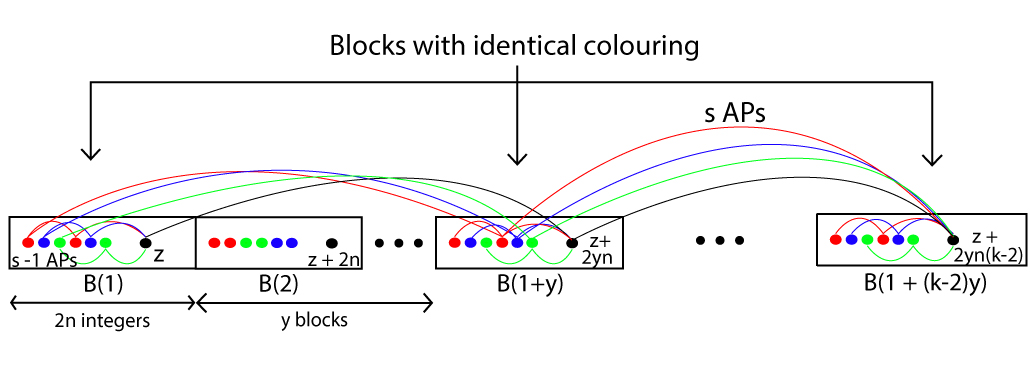
\includegraphics[scale=1.8]{Figuras/Van-der-Waerden-Blocks.jpg}
     \caption{s APs in the $W(r^{2n},k-1)$ blocks.}
     \label{fig:VanderWaerdenBlocks}
\end{figure}

The theorem follows from the claim by setting $s=r$ because if we have $s$  APs colour focused at $z$ there is no other different colour to use in $z$, by the fact all AP has length $k-1$  independent the colour we choose for $z$ we will have a AP with length $k$.

\end{proof}



\chapter{Extremal Graph Theory}
In this chapter, the problems and theorems extend previous chapter. Instead of working only in questions based on sets' cardinality it embraces questions about the maximum size of graphs and graphs' substructures.
\section{Turán's Theorem}
In this section we study prohibited subgraphs to answer questions of the following form: 
\begin{center}``What is the maximum number of edges in a tringle-free graph?''\end{center}
As we see in the next theorem the complete bipartite graph has $\frac{n^{2}}{4}$ edges and no triangles.\\
\begin{theorem}
(Mantel, 1907). If G is a triangle-free graph on $n$ vertices, then 
$$e(G) \leq \left\lceil \frac{n}{2} \right\rceil \left\lfloor \frac{n}{2} \right\rfloor .$$
\end{theorem}
\begin{proof}
This is a proof by induction on $n$. Let $G'$ be the graph obtained from $G$ by removing two vertices $\{u\},\{v\} \in G$ such that $\{uv\}\in e(G)$, note that if $G$ is triangle-free so $G'$ is also triangle-free because it is not possible to form a triangle removing a edge and there are at most $n-1$ edges incident with $u$ or $v$, then:
\begin{align*}
e(G-\{\{u\},\{v\}\}) &\leq (\left\lfloor \frac{n}{2} \right\rfloor -1)(\left\lceil \frac{n}{2} \right\rceil -1) \\
&= \left\lfloor \frac{n}{2} \right\rfloor \left\lceil \frac{n}{2} \right\rceil - n +1.
\end{align*}
When we add the $n-1$ edges removed from $G$ we confirm the induction hypothesis. 
\end{proof}

Turán generalized its result in 1941. We will need following definitions: 
\begin{definition}$T_r(n)$ is the complete $r$-partite graph with $n$ vertices and $\left\lceil \frac{n}{r} \right\rceil$ or $\left\lfloor \frac{n}{r} \right\rfloor$ vertices on each part and it is called the Turán's graph.
\end{definition}

\begin{definition}
$t_r(n)$ is the number of edges in the Turán's graph, then $e(T_r(n)) = t_r(n)$ and it is called Turán's number.
\end{definition}

\begin{theorem} \label{theorem:turan1941}(Turán, 1941). $ex(n, k_{r+1}) = t_r(n)$ and $T_r(n)$ is the only extremal graph.
\end{theorem}

\begin{proof}
This is a proof by induction on $n$. Note $d(v) \approx n-(n/r)$ with $v \in V(G)$ and $G$ being the complete $r$-partite graph. Now, using the fact $\sum_{v\in V(G)} d(v) = 2 e(G)$ follows:

$$ t_r(n) \approx \frac{n}{2}\left(n-\frac{n}{r}\right) \approx \left(1-\frac{1}{r}\right) \binom{n}{2}.$$


 Let $G$ be maximum without a $K_{r+1}$. Construct a graph $G'$ removing a $K_r$ from $G$ as Figure \ref{fig:G'andKr}. Note that each vertex in $G'$ could be neighbour of at most $r-1$ vertices in $K_r$, otherwise $G$ would have a $K_{r+1}$, then we have $(r-1)(n-r)$ vertices between $G'$ and $K_r$.
 
 \begin{figure}[H]
     \centering
     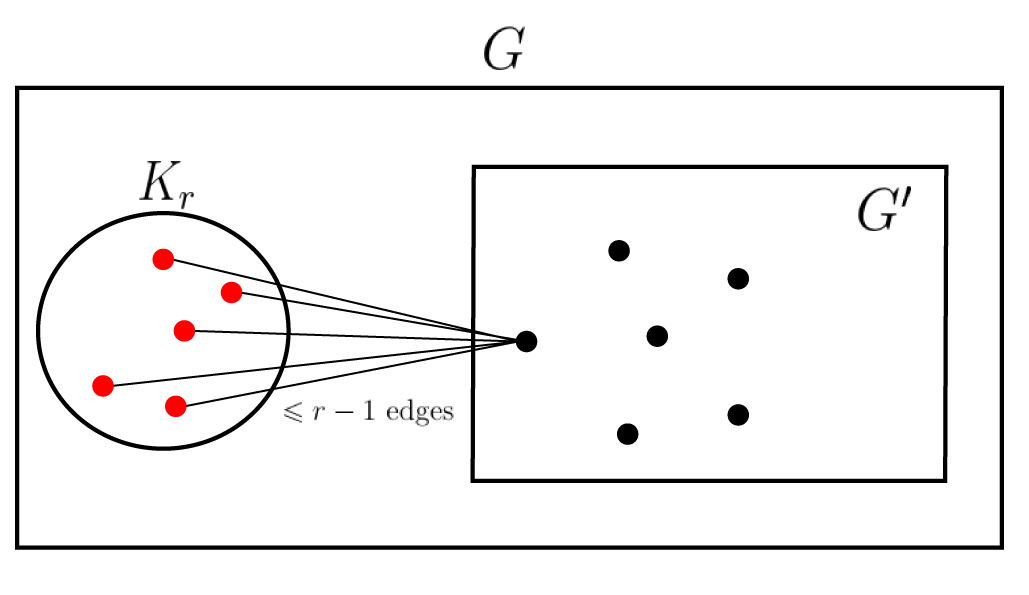
\includegraphics[scale=1]{Figuras/Kr+1-livre-prova-turan.jpg}
     \caption{$G'$ and $K_r$.}
     \label{fig:G'andKr}
\end{figure}

Note inside the $K_r$ there exists $\binom{r}{2}$ edges and by induction hypothesis we have $e(G') \leq t_r(n-r)$, then follows:

\begin{align*}
e(G) &\leq e(G') + (r-1)(n-r) + \binom{r}{2}\\
&\leq t_r(n-r) +(r-1)(n-r) + \binom{r}{2}\\
&= t_r(n).
\end{align*}

The last line comes from the fact $t_r(n) - t_r(n-r) = \binom{r}{2} + (r-1)(n-r)$ as we can see at Figure \ref{fig:t(n)-and-t(n-r)} removing a vertex of each part we remove $\binom{r}{2}$ edges between the $r$ vertices removed and $(r-1)(n-r)$ edges  bacause every vertex in $T_r(n)$ is connected exactly with $r-1$ vertices of the $r$ vertices removed.   

 \begin{figure}[H]
     \centering
     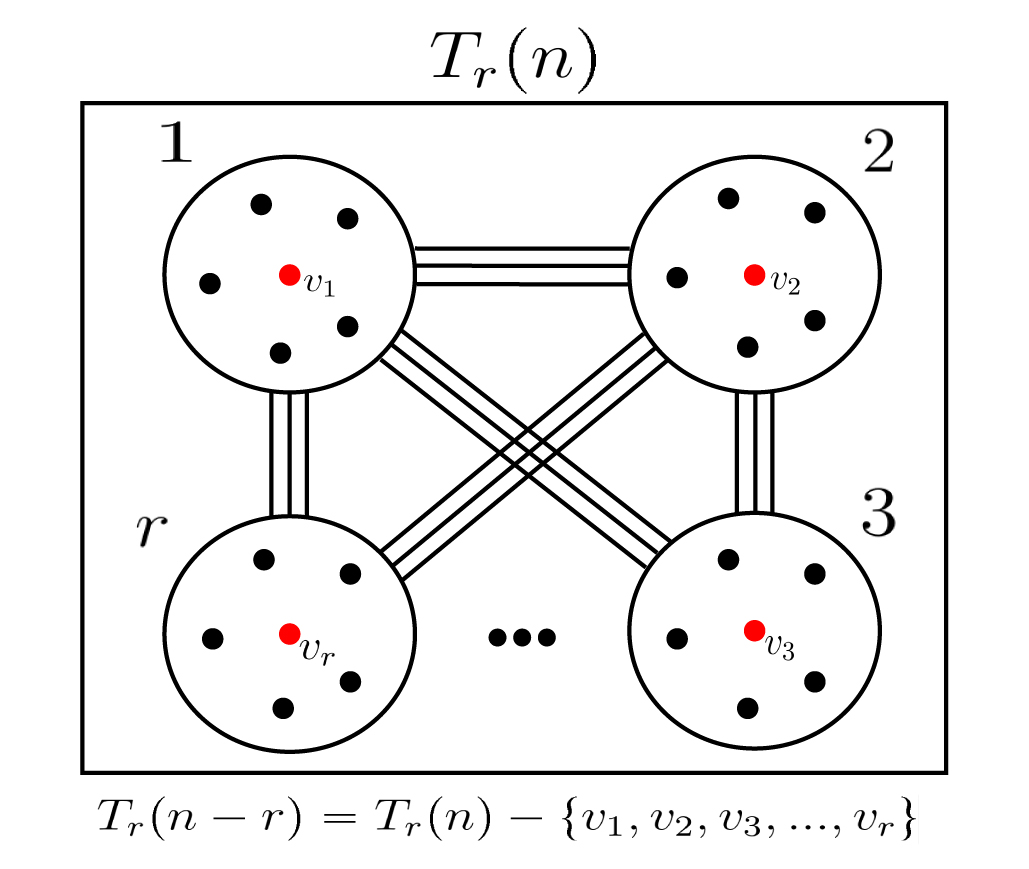
\includegraphics[scale=1]{Figuras/t(n)-and-t(n-r)}
     \caption{$T(n)$ and $T(n-r)$.}
     \label{fig:t(n)-and-t(n-r)}
\end{figure}
Then the proof is finished.
\end{proof}

\begin{theorem}\label{theorem:erdos1970} (Erd\H{o}s, 1970). There is an $ r$-partite graph $H$ with $V(H) = V(G)$, with $d_H(v) \geq d_G(v)$ for every $v \in V(G)$.\\
\end{theorem}

\begin{proof}
 Let $G$ be a $ K_{r+1}-$free graph on $n$ vertices and let $w$ be a vertex of maximum degree in $G$. For every vertex $v \in V(G)\setminus N(w)$ is removed the edges incident with v and added an edge between $v$ and each neighbor of $w$, this operation is called `Zykov symmetrization'. Clearly, no vertex degree has decreased because at this point $d(v) = \Delta(G)$ for every $v \in V(G)\setminus N(w)$ and the graph is still $K_{r+1}-$free because $N(w)$ has not changed and the $G\setminus N(w)$ is a independent set now.

Being $w\in V(G)$ a vertex of maximal degree in $G$, note that $H=G[N(w)]$ must be $K_r-$free by our graph choice (otherwise $G$ would not be $K_{r+1}-$free). So by induction hypothesis, exists a $(r-1)-$partite graph $H_1$ on $N(w)$ with $d_{H_1}(v) \geq d_{H}(v)$ for every $v \in N(w)$. Let $G_1$ be the graph obtained from $G$ by performing Zykov symmetrization at vertex $w$. Now replace $H$ by $H_1$ and we acquire $G_1$ which is the required $r-$partite graph, note it is valid because in any step the degrees have decreased.
\end{proof}
This theorem is related to Theorem \ref{theorem:turan1941}. In fact Theorem \ref{theorem:erdos1970} is stronger than Theorem \ref{theorem:turan1941} and we can see this relation as follows: $$e(G) \leq e(H) \leq e(T_r(n)).$$
\section{Forbidden Bipartite Subgraphs}
In this section we study what the consequences when small bipartite graphs are forbidden and starts with Jensen's inequality for convex functions because its importance for a next Erd\H{o}s' result in Theorem \ref{theorem: Erdos,1938}.
\begin{proposition}\label{prep:jensen}
(Jensen's Inequality). If $0\leq \lambda_i \leq 1, \sum_{i=1}^n \lambda_i = 1$ and $f$ is convex, then:

$$
f \left( \sum_{i=1}^n \lambda_i x_i\right) \leq \sum_{i=1}^n \lambda_i f (x_i).
$$

\end{proposition}

As showed in previous chapter, thus Theorem \ref{theorem:turan1941}:
$$ ex(n,K_{r+1}) = e(T_{r,n}) \approx \left( 1-\frac{1}{r}\right) \binom{n}{2} .$$
Erd\H{o}s proved that the extremal number is much smaller for the $4$-cycle graph.
 
\begin{theorem} \label{theorem: Erdos,1938}
(Erd\H{o}s, 1938).

$$\text{ex}(n,C_4) = O(n^{3/2}).$$
\end{theorem}

\begin{proof}
A $C_4$ is formed by two `cherries' in the same pair of vertices. Counting these triples (x,\{y,z\}) of distinct vertices in G such that $xy, xz \in E(G)$ and using proposition \ref{prep:jensen} with $\lambda_i = 1/n$ we obtain a very useful inequality,

$$ \sum_{i=1}^n \frac{1}{n} f\left(x_i\right) \geq f\left(\sum_{i=1}^n \frac{1}{n} x_i\right),$$
using our convex function,
$$ \frac{\sum_{i=1}^n \binom{x_i}{2}}{n} \geq \binom{\frac{\sum_{i=1}^n x_i}{n}}{2} ,$$
replacing $x_i$ and assuming $\sum_{v \in V(G)} d(v) = 2e(G),$

\begin{align*}
\sum_{v \in V(G)} \binom{d(v)}{2} &\geq n \binom{\frac{2e(G)}{n}}{2}\\
&= n\frac{\frac{2e(G)}{n}\left( \frac{2e(G)}{n}-1\right)}{2} \\
&\geq \frac{n}{2} \left( \frac{2e(G)}{n} - 1 \right)^2.
\end{align*}
And since the maximum number of such triples in a $C_4$-free graph is at most $\binom{n}{2}$ because we can have only one cherry for each pair of vertices,
$$ \frac{n}{2}\left(\frac{2e(G)}{n} - 1\right)^2 \leq \binom{n}{2},$$
we obtain $e(G) = O(n^{3/2})$ finishing the proof.
\end{proof}

Let $A = \{a_1,...,a_t\} \subset [n]$ be such that $a_ia_j \neq a_ka_l$ unless $\{i,j\} = \{k,l\}$. How big can be $A$ with these properties?
To show a easy lower bound it is necessary only a example that fits the problem, for this problem we can use the number of primes in $[n]$ which is $\pi (n)$. But is it close to the maximum possible size?

Erdos used theorem \ref{theorem: Erdos,1938} to answer this question.

\begin{corollary}(Erd\H{o}s, 1938). Let $A\subseteq [n]$ be a multiplicative Sidon set. Then,
$$ |A| \leq \pi(n) + O(n^{3/4}). $$

\end{corollary}
The next result is very similar to theorem \ref{theorem: Erdos,1938}. In fact, it is a generalization of Erd\H{o}s' result, but instead counting cherries we count generalized cherries.
\begin{theorem}(Kovari-Sós-Turán, 1954). If $s \leq t$, then
$$ ex(K(s,t)) = O (n^{2 - 1/s}). $$
\end{theorem}

\begin{proof}

At this proof we do a double counting on generalized cherries, a generalized cherry is a vertex with a fixed number of neighbors as you can see at figure \ref{fig:generalizedcherry}

\begin{figure}[!htb]
     \centering
     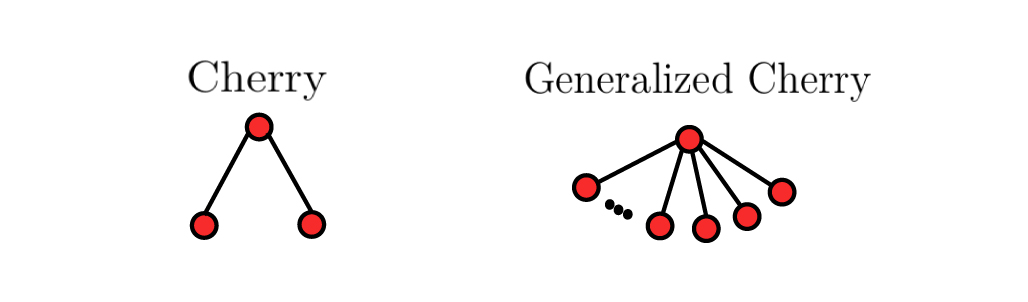
\includegraphics[scale=1]{Figuras/generalized-cherry.jpg}
     \caption{Cherry and Generalized Cherry.}
     \label{fig:generalizedcherry}
\end{figure}

$K_{1,s}$ is the generalized cherry we need to count. Note we can count it by taking all possible sets of $s$ neighbors of each vertex, as follows,
$$ \# K_{1,s} = \sum_{v \in V(G)} \binom{d(v)}{s} .$$

Now we use the fact $\left(\frac{n}{m}\right)^m \leq \binom{n}{m} \leq \left(\frac{en}{m}\right)^m$ and Jensen's Inequality \ref{prep:jensen} to acquire the following inequality,

\begin{align*} 
\sum_{v \in V(G)} \binom{d(v)}{s} & \geq \sum_{v \in V(G)}\frac{d(v)^s}{s^s}\\ 
& \geq \frac{1}{s^s} n \left( \frac{\sum_{v \in V(G)} d(v)}{n} \right) ^s \\
& = \frac{1}{s^s} n \left( \frac{ 2 e(G)}{n} \right) ^s \\
& \geq c(s) \frac{e(G)^s}{n^{s-1}},
\end{align*}
where $c(s) = \left(\frac{2}{s}\right)^s$.
We already have a lower bound for $K_{1,s}$ that depends of the number of edges, now let's construct a upper bound counting the maximum number of generalized cherries.
As $K(s,t)$ is the complete bipartite graph with two partitions whose sizes are $|s|$ and $|t|$ we know the maximum number of $K_{1,s}$ is $t\binom{n}{s}$ but since we want the extremal number of edges without a $K_{s,t}$ we have,

\begin{align*}
c(s) \frac{e(G)^s}{n^{s-1}} &\leq \# K_{1,s} \leq (t-1) \binom{n}{s}\\
		       & \Rightarrow e(G)^s \leq \frac{1}{c(s)}\frac{e(t-1)}{s^s}n^{2s-1}\\
		       &\Rightarrow e(G) \leq c(s,t) n^{2-1/s}\\
		       &\Rightarrow e(G) = O(n^{2-1/s}),
\end{align*}
Where $c(s,t)= \sqrt[s]{\frac{1}{c(s)}\frac{e(t-1)}{s^s}}$ . Using again the fact $\binom{n}{m} \leq \left(\frac{en}{m}\right)^m$ we have what we want to show and the proof is finished.
\end{proof}

\section{The Erd\H{o}s-Stone Theorem}
This theorem is extremely important for graph theory and can be called as the fundamental theorem of graph theory such its importance. To prove it we need the following definition.
\begin{definition} The Chromatic Number:
$$\chi(G) = \text{ min}\{r: \exists c : V(G) \rightarrow [r] \text{ such that } c(u) \neq c(v) \text{ for every } uv \in E(G)\}$$ 
\end{definition}

Note $\chi(G)$ is related to $r$-partite graphs, a graph $G$ is $r$-partite if and only if $\chi(G) \leq r$.


\begin{theorem}
(Erd\H{o}s and Stone, 1946). Let H be an arbitrary graph. Then
$$ ex(n,H) = \left(1-\frac{1}{\chi (H)-1} + o(1)\right) \binom{n}{2}.$$ 
\end{theorem}

\begin{proof}

Here will be the proof.

\end{proof}

\chapter{Random Graphs}
\section{The Probabilistic Method}
This method is very powerful and has incredible simple applications, when this method begun to being used it created many shocking proofs, but not all applications of the method are so simple or easy to understand. A central fact for the probabilistic method is ``a object with property $ A$ exists $\iff  \mathbb{P}(\text{object has property }A)>0$''

It is necessary to introduce the Erd\H{o}s-Rényi random graph $G(n,p)$ which although the name is not a graph. $G(n,p)$ is a probability distribution on graphs, more informally, it is a edge distribution on n vertices with probability p and with the existence of edges being independent events.

\begin{definition}\label{def:randomgraph}
The (Er\H{o}s-Rényi) random graph, $G(n,p)$, is the graph on $n$ vertices obtained by choosing each edge independently at random with probability $p$. In other words, we assume that we have a probability space $\Omega$ and independent random variables $I_{vw}$ for each $vw \in \binom{[n]}{2}$, such that
$$\mathbb{P}(I_{vw} = 1) = 1 - \mathbb{P}(I_{vw} = 0),$$ 
and let $G$ be the graph with vertex set $[n]$ and edge set $\{vw \in \binom{[n]}{2}: I_{vw} = 1\}$. 

\end{definition}

%$$\mathbb{P}(e \in E(G(n,p)))=p ,$$ \\and\\$$ 1-p=\mathbb{P}(e \notin E(G(n,p))),$$

{\bf Question:} What is the probability of $G(n,p) = H$, with $H$ being a fixed graph?
Intuitively we can guess there exists a really small chance that this event occurs and the intuition in this case is true, let's see this probability below,
$$\mathbb{P}(G(n,p)=H) = p^{e(H)}(1-p)^{\binom{n}{2}-e(H)}.$$

\begin{theorem}(Erd\H{o}s, 1959) There exist graphs whose girth and chromatic number are both arbitrarily large.
\end{theorem}

For this theorem will be presented two different proofs, the second one is a little smaller.

\begin{proof} First proof.
In other words, we need to prove:

$$\mathbb{P}\binom{\chi(G(n,p)) \geq k \text{ and }} {g(G(n,p)) \geq k} > 0 ,$$
for some $p =p(n) \in (0,1)$ and a sufficiently large $n$.

First of all, we need some definitions,
\begin{definition}\label{def:girth}
$g(G)$ is the girth of $G$ which is the length of the shortest cycle in $G$. 
\end{definition}
\begin{definition}\label{def:independencenumber}
$\alpha(G) =$ max$\{|A|: A$ is a independent set$\}$.
\end{definition}
\begin{definition}\label{def:chromaticnumber}
$\chi(G)$ is the minimum number of colors used in a proper coloring of G.
\end{definition}
Assuming $\chi(G(n,p)) = r$ we have a $\{V_1,V_2,...,V_r\}$ partition of $V(G(n,p))$ on $r$ independent sets illustrated at figure \ref{fig:r-partition}

\begin{figure}[!htb]
     \centering
     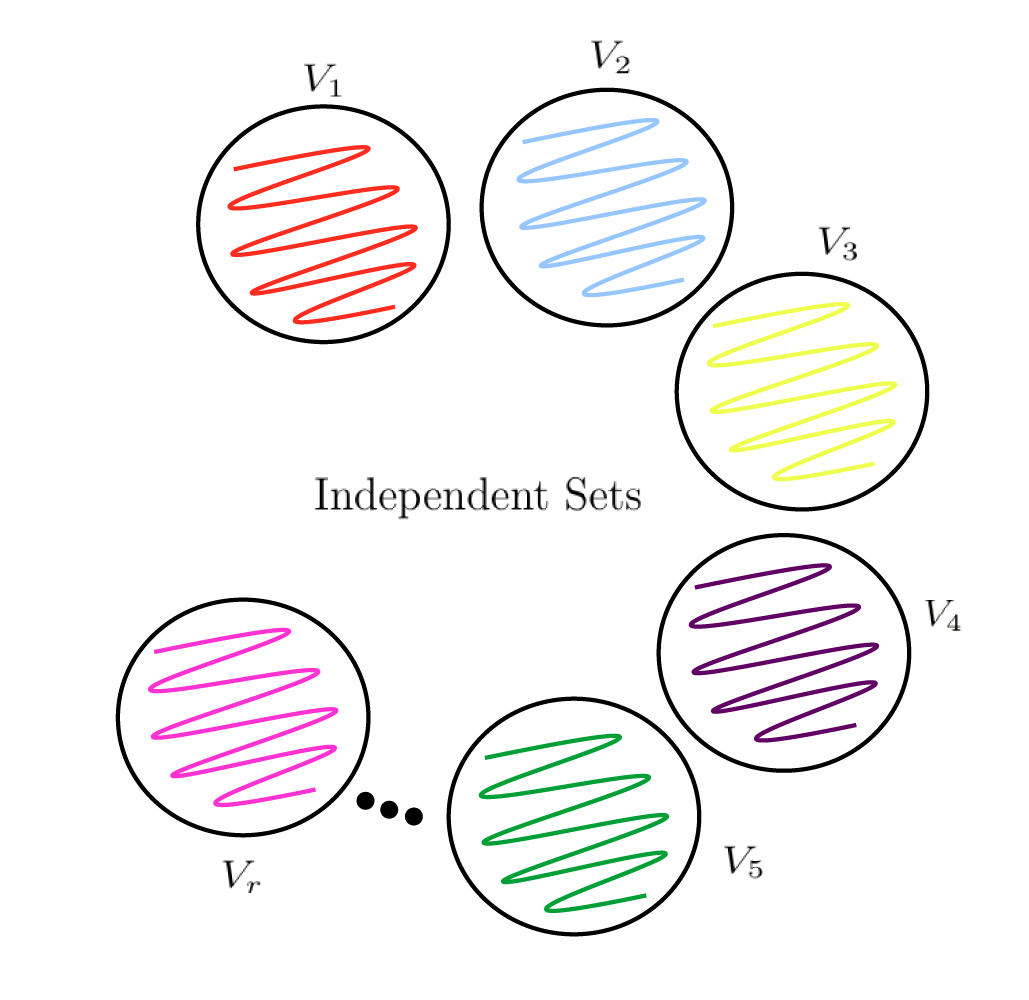
\includegraphics[scale=1]{Figuras/r-partion.jpg}
     \caption{r-coloring partition. }
     \label{fig:r-partition}
\end{figure}

By the pigeonhole principle we have $\alpha (G) \geq \frac{n}{r}$ and since $\chi(G)=r$,

$$\chi(G(n,p)) \geq \frac{n}{\alpha(G(n,p))},$$

and we want to show:

$$\chi(G(n,p)) \geq \frac{n}{\alpha(G(n,p))} \geq k ,$$

Then,

$$\alpha(G(n,p)) < m \iff X_m=0 ,$$
with 
%$X_m = \{|[A]|: S \in A$ if $S$ is a independent set with at least $m$ elements in $G(n,p)\}$,
$X_m = \big|\{S\in V(G(n,p))\colon \text{$S$ is a independent set with exactly $m$ vertices in $G(n,p)$}\}\big|$,
and follows $m = \frac{n}{k}$. 

\begin{align*}
\mathbb{E}[X_m]&=\sum_{\substack{S \in V(G) \\ |S| = m}} \mathbb{P}(S\text{ is independent })\\
&=(1-p)^{\binom{m}{2}} \binom{n}{m}
\end{align*}
since we know that $\left(\frac{n}{m}\right)^m \leq \binom{n}{m} \leq \left(\frac{en}{m}\right)^m$ and $1-x \leq e^{-x}$ replacing in the equation above,
\begin{align*}
\mathbb{E}[X_m] &\leq \left(\frac{en}{m}\right)^m  e^{(-pm^2)} \\
&= \left(\frac{en}{m} e^{(-pm)}\right)^m\\
&\leq \left(\frac{en}{m} e^{(-pm)}\right)^m \\
&= \left(\frac{en}{m}\frac{1}{e^{(pm)}}\right)^m  \\
&\ll 1 \text{ if } e^{pm} \gg n
\end{align*}

remember $m =\frac{n}{k}$ and using a logarithm function on both sides of equation to isolate $p$,

$$ pn/k \gg \log n \Rightarrow p \gg \frac{k\log n}{n},$$
 
 By Markov's inequality,
 
 $$ \mathbb{P}(X_m \geq 1) \leq \mathbb{E}[X_m] ,$$
 
and if $p \gg \frac{k \log n}{n}$ we have,
 
 \begin{align*}
\mathbb{P}(X_m \geq 1) &\leq \mathbb{E}[X_m] \\
&\leq \frac{1}{100}  \\
&\Rightarrow \mathbb{P}(\alpha (G(n,p)) < \frac{n}{k}) \geq \frac{99}{100}\\ 
&\Rightarrow  \mathbb{P}(\chi(G(n,p)) > k) \geq \frac{99}{100}.
\end{align*}

Since the proof for $\chi(G) \geq k$ is finished we will prove $g(G(n,p))\geq k$,

$$ g(G(n,p)) \leq k \iff X_k \geq 1,$$


where $X_k = \#  C_k$ in $G(n,p)$,

$$\mathbb{E}[X_k] = \sum_{C_k \subset K_n} \mathbb{P}(C_k \subset G(n,p) ) \leq n^kp^k,$$

now we need to limit our short cycles by $\sqrt{n}$ in order to show with high probability we will have few short cycles so we can destroy then without changing anything,

$$n^kp^k \leq \sqrt{n} \text{ if } p \leq n^{-1 + \frac{1}{2k}},$$

then getting together with our previous result,

$$\frac{k\log k}{n} \ll p \leq n^{-1 + \frac{1}{2k}}.$$

And we can remove a vertex of each cycle with length $<k$, so we have $g(G) \geq k$. Note removing a cycle's vertex doesn't make $\alpha(G)$ bigger and consequently doesn't make $\chi(G)$ smaller, maintaining all our previous calculations valid.
\end{proof}

\begin{proof}
Second Proof. Using the same definitions of the first proof for girth \ref{def:girth}, independence number \ref{def:independencenumber} and chromatic number \ref{def:chromaticnumber} we have,

$$ |G| = \sum_{i=1}^{\chi(G)} |S_i| \leq \chi(G)max|S_i| \leq \chi(G) \alpha (G) .$$

Note that if $\alpha(G) \leq |G|/k$, then $\chi(G) \geq $k. \\
Let $\epsilon > 0$ be sufficiently small ($\epsilon < 1/k$) and $p = n^{\epsilon - 1}$. As we have already been introduced to $G(n,p)$ in definition \ref{def:randomgraph} let $G = G(n,p) -$\{one vertex of each cycle $C_l \text{ with } l\leq k\}$.

Now we need two claims to reach the result. We claim that, with high probability, $G$ has at most $n/2$ cycles of length $\leq k$ and has no independent set  of size $n/2k$ then, consequently $\chi(G) \geq k$ and $girth(G) \geq k$.

First claim. $V(G) > n/2$ . First of all we need some variables to count the cycles,
$$X_l = \# C_l \subset G(n,p)$$
$$X = \# \text{ short cycles } = \sum_{l=3}^k X_l$$
\begin{align*}
\mathbb{E}[X] &= \sum_{l=3}^k \mathbb{E}[X_l] \\
	       &= \sum_{l=3}^k \sum_{C_l \in K_n} \mathbb{P}(C_l \subset G(n,p))\\
	       &\leq \sum_{l=3}^k n^l p^l \\
	       &= \sum_{l=3}^k n^{\epsilon l}, p= n^{\epsilon - 1}\\
	       &\leq 2n^{\epsilon k} \\
	       &= o(n).
\end{align*}
Note that since we are removing a vertex of each cycle $V(G) \geq n-X$. Now we show the general case for this important inequality for the probabilistic method. The Markov's inequality holds for any random variable which takes non-negative valuers and for $a>0$,

$$\mathbb{P}(X>a) \leq \frac{\mathbb{E}(X)}{a}.$$

Using it and replacing $\mathbb{E}[X]$ by its upper bound we have,

\begin{align*}
\mathbb{P}(X\geq n/2) &\leq \mathbb{E}[X]/(n/2)\\
		& = o(n)/n\\
		& = o(1)
\end{align*}
Then, we proved that, with high probability, we don't have more than $n/2 -1$ cycles with length at most $k$ and consequently we have $V(G) > n/2$ .\\
\\
Second claim. $\alpha(G) \leq \alpha (G(n,p)) < n/2k$.\\
We need to count the independent sets,
$$Y_l = \# \text{ independents sets with length $l$. }$$

\begin{align*}
\mathbb{E}[Y_l] &= \sum_{\substack{|S| = l \\ e(S) = 0 }} (1-p)^{\binom{l}{2}}\\
	       &= (1-p)^{\binom{l}{2} \binom{n}{l}} \\
	       &\leq \left(\frac{en}{l}\right)^l e^{-p\binom{l}{2}}\\
	       &\rightarrow 0  \text{ if } l = n/2k.
\end{align*}

Thus both claims,

$$\frac{\mathbb{E}[|\{C_l \subset G : l\leq k \}|]}{n/2} + \mathbb{E} [|\{ S:|S| \geq n/2k, e(S) = 0\}|] \rightarrow 0$$
as $n \rightarrow \infty $. So $G$ has the desired properties with high probability and the prove is finished.
\end{proof}

Realize that the key point in both proofs was the fact we could choose the most comfortable probability distribution, what gives us a huge flexibility to construct proofs.

\section{The Janson and FKG Inequalities}

At this section we will focus on the occurrence of  bad events, asking questions as the form ``Could we count the number of bad events?'' or ``What is the probability that none of the bad events occurs?''. The Janson and FKG inequalities give us tools to answer this type of question.

\subsection{The FKG inequality}

\begin{definition}
Monotone Increasing. Let $\mathcal{A}$ be a collection of graphs on $n$ vertices, $\mathcal{A}$ is monotone increasing if $G \in \mathcal{A}$ and $e(G) \subset e(H)$ implies $H \in \mathcal{A}$, so if $G \in \mathcal{A}$ this means adding edges doesn't make $G$ loose the characteristics that makes it be in $\mathcal{A}$ and it is called monotone decreasing otherwise.     
\end{definition}

\begin{example}
``$G$ contains a triangle'' is monotone increasing because it is impossible to destroy a triangle adding edges and ``$G$ is planar'' is monotone decreasing because the more edges $G$ has more difficult to be planar.
\end{example}

\begin{theorem} (FKG inequality).
 Let $\mathcal{A}$ and $\mathcal{B}$ be monotone increasing and let $\mathcal{C}$ be monotone decreasing, then:

$$ \mathbb{P}((G_{n,p} \in \mathcal{A}) \wedge (G_{n,p} \in \mathcal{B})) \geq \mathbb{P}(G_{n,p} \in \mathcal{A})\mathbb{P}(G_{n,p} \in \mathcal{B}),$$
and
$$ \mathbb{P}((G_{n,p} \in \mathcal{A}) \wedge (G_{n,p} \in \mathcal{C})) \leq \mathbb{P}(G_{n,p} \in \mathcal{A})\mathbb{P}(G_{n,p} \in \mathcal{C}).$$
\end{theorem}

\subsection{Janson's Inequality}

\subsection{Nameless Section}
\begin{theorem}
Let $c$ be a constant and $p = \frac{c}{n}$. Then

$$ \limsup_{n \rightarrow \infty}\mathbb{P}(G_{n,p}\text{ contains a triangle }) = 1 - e^{\frac{-c^3}{6}}.$$
\end{theorem}

%\section{Subgraphs of the Random Graph}

\chapter{Regularity}

\chapter{Schedule}

\begin{table}[h]
\centering

\begin{tabular}{|r|lr|}
\hline
Task & Month&Year \\ 
\hline                               
Chapter 1& September & 2018 \\
Chapter 2 &October & 2018 \\
Chapter 3&November & 2018 \\
 &December & 2018 \\
Chapter 4&January & 2019 \\
Chapter 5&February & 2019 \\
Conclusion&March & 2019 \\
Defense&April & 2019 \\
 &May & 2019   \\ 
\hline
\end{tabular}
\caption{Schedule.}
\label{tab:schedule}
\end{table}

\end{document}

%%% Local Variables:
%%% mode: latex
%%% eval: (auto-fill-mode t)
%%% eval: (LaTeX-math-mode t)
%%% eval: (flyspell-mode t)
%%% TeX-master: t
%%% En